\documentclass[aspectratio=43]{beamer}

% Pakete für das Dokument
\usepackage{blindtext}
\usepackage{../../inc/beamerthememnrstyle}

\usepackage{caption}
\captionsetup{justification   = raggedright,
              singlelinecheck = false}
% Eigenes Theme laden
\usetheme{mnrstyle}

% Eigene Definition von enumerate
% \setlist[enumerate, 2]{label=\roman*., format=\itshape, leftmargin=2cm}

% Metadaten für das Dokument
\title{Die Bibel}
\author{\MakeUppercase{Lothar Schmid}}
\date{2025}
\begin{document}

% Titelframe
\begin{frame}
    \maketitle    
\end{frame}
\begin{frame}
    \frametitle{Übersicht}  % Frametitel
    \begin{enumerate}
        \item \textbf{Ein Buch -- 2022 mehr als 35 Mio Biblen}
        
        \item \textbf{\color{gray}Ein Buch -- mit 1200 - 1400 Seiten}
      
        \item \textbf{\color{gray}Ein Buch -- 2023 3686 Sprachen übersetzt\\
        (in 743 Sprachen die ganze Bibel)}
                         
    \end{enumerate}   
\end{frame}

% Frametitel setzen
\begin{frame}
    \frametitle{Der Beginn}  % Frametitel
    \begin{columns}
        \begin{column}{0.5\textwidth}
            \begin{figure}[t]
                \centering
                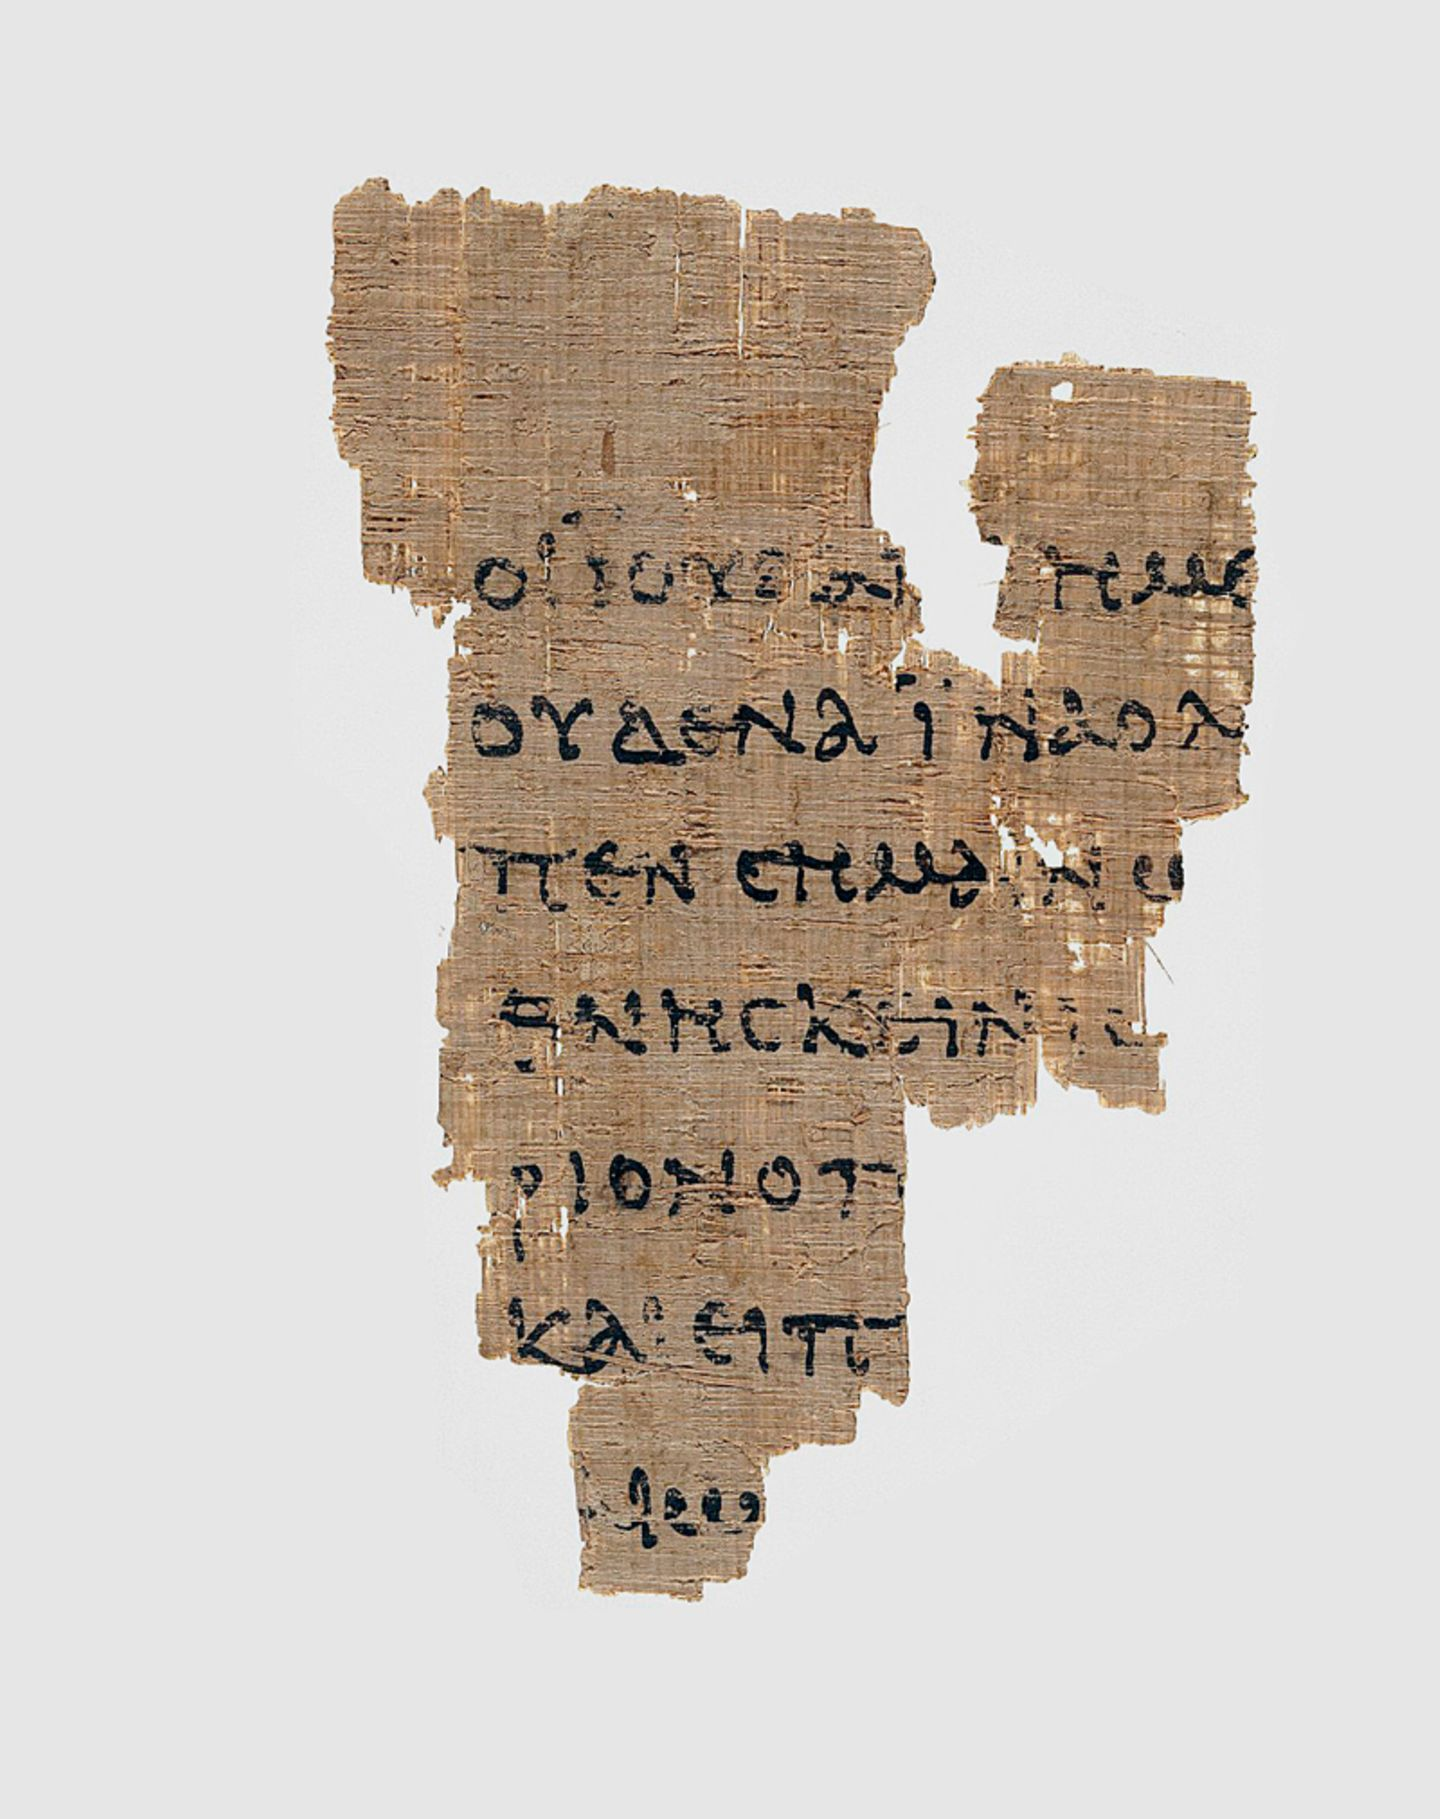
\includegraphics[width=0.5\linewidth]{src/Vorträge/BibelBuch/images/papyrusFragment.jpg}
                \caption{{ \textcopyright John Rylands Library}}
                \label{fig:enter-label}
            \end{figure}
        \end{column}
        \begin{column}{0.5\textwidth}
            \small Dieses Papyrusfragment von etwa 125 n. Chr. ist der älteste Beleg für das Neue Testament. Er handelt vom Prozess gegen Jesus: Die Frage »Bist du der König der Juden?« ist teilweise zu entziffern\\
        \end{column}
    \end{columns}
\end{frame}
%%%%%%%%%%%%%%%%%%%%%%%%% Folie 3 %%%%%%%%%%%%%%%%%%%%%%%%%%%%%%%%
\begin{frame}
    \frametitle{Über Gott und den Menschen}  % Frametitel
    \begin{enumerate}
        \item \textbf{Der eine ewige und vollkommene Gott}
            \begin{itemize}              
                \item Gott ist der Schöpfer aller Dinge und existiert ewig in drei Personen: Vater, Sohn und Heiliger Geist.
            \end{itemize}
            \vspace{0.25cm}
        \item \textbf{Der Mensch und die Schöpfungsordnung Gottes}
            \begin{itemize}
                \item Der Mensch wurde nach Gottes Bild geschaffen, doch die Sünde brachte Trennung von Gott und Unordnung in die Schöpfung.
            \end{itemize}
            \vspace{0.25cm}
        \item \textbf{Jesus Christus: Gottes Sohn und unser Erlöser}
            \begin{itemize}
                \item Jesus Christus wurde Mensch, nahm die Sünden der Welt auf sich und wurde durch Seine Auferstehung zum Weg der Erlösung.
            \end{itemize}              
    \end{enumerate}   
\end{frame}


\end{document}
